% !TEX root = main.tex

\section{はじめに}
現在のコンピュータ技術は複数のコアを用いて処理を行うマルチスレッド処理が主流であり,近年では単体で200コアを超えるマシンも登場し始めている.
データベース分野においても,メニーコアなどを前提としたインメモリデータベースの研究が進んでいる.
データベースの構成要素の1つである索引技術も同様に,メニーコア化したCPUの限活用が求められている.

代表的な索引構造である\Bptree{}~\cite{book:dbsystem}においても,メニーコアを有効利用するための同時実行制御手法が提案されている.
伝統的なデータベースでは\Bptree{}の制御にロックが使用されるが,マルチスレッド処理においてロックによる同時実行制御は多数の待ちスレッドが発生しうるため,スケーラビリティを悪化させる.
そのため,\Bptree{}をロックフリー化させた索引としてBw木~\cite{book:Bwtree}やBz木~\cite{book:Bztree}が提案された.
更に,それらを凌ぐ書き込み性能を達成する索引として著者らの研究室でも同時実行\Bptree{}(concurrent-\Bptree{}, \Bctree{}~\cite{deim:Hirano2024})を開発している.

\Bctree{}を含め,\Bptree{}を基にした索引は可変長データを始めとする任意のデータ型を格納可能な汎用的な索引構造であるが,一方で特定のデータ型への特化による性能改善も可能である.
例えば,キーをバイナリ比較可能なデータ型に限定することで性能を改善したものとしてMass木~\cite{book:Masstree}がある.
Mass木では,キーがバイナリ比較可能であるため,キーを先頭から8~byte単位で分割し各部分キーで\Bptree{}を構成する.
これにより\Bptree{}内で管理されるキーが固定長となるため,キャッシュ効率に優れたノード構成を適用できる.
更に,部分キーによる階層構造はトライ木の構造と同様であり,先頭で一致したキーの共有によるキャッシュ効率の改善も可能である.

\begin{figure}[t]
    \centering
    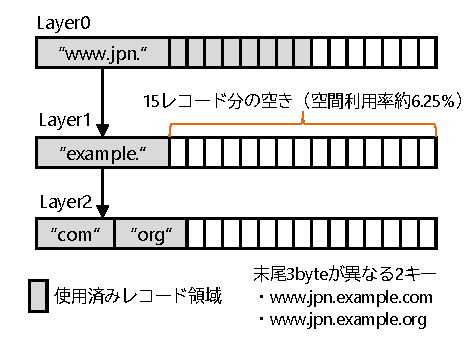
\includegraphics{./figures/mass_memory.pdf}
    \caption{Mass木の空間利用率}
    \label{fig:memory}
\end{figure}

しかし,Mass木においては空間利用効率が問題となる.
\Fig{\ref{fig:memory}}は末尾3~byteが異なる19~byteの2~キーを格納したMass木の索引構造である.
先頭8~byteが共通するため,layer~1を作成する.
同様に8~16~byte目が共通するため,layer~2を作成する.
Mass木では本来,1~つのノードに最大16~個のレコードを格納できる.
しかしlayer~1では,1~つのレコードしか格納されていない状態でlayer~2を作成している.
layer~1にのみ注目すると,空間利用率は約6.25~\%しかない.

そこで本研究では,\Bctree{}に対し扱うキーをバイナリ比較可能な型に限定することで性能を改善するとともに,Mass木のようなメモリ効率の悪化を回避した索引構造である\Bcforest{}を提案する.
\Bcforest{}の概形を\Fig{\ref{fig:bcforest}}に示す.
Mass木と同様に\Bctree{}を階層的に作成することおよび中間ノードのノード構成を特化させることで,キャッシュ効率を改善する.
また,葉ノードにおけるPosting listの利用により,Mass木における空間利用率の改善を図る.

\begin{figure}[t]
    \centering
    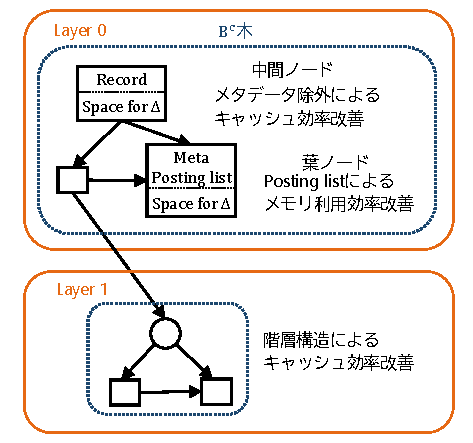
\includegraphics{./figures/bcforest.pdf}
    \caption{\Bcforest{}の概形}
    \label{fig:bcforest}
\end{figure}

本稿の構成は以下の通りである.
\Sec{\ref{sec:relatedwork}}では,関連研究としてロックフリー索引やバイナリ比較可能なキーに対し最適化した索引について概説する.
次に,\Sec{\ref{sec:bc_forest_structure}}で\Bcforest{}の構造について説明し,\Sec{\ref{sec:node_operation}}および\Sec{\ref{sec:smo}}で\Bcforest{}の操作について述べる.
最後に,\Sec{\ref{sec:conclusion}}で本稿のまとめと今後の方針を述べる.

\section{関連研究}
\label{sec:relatedwork}
関連の深い索引構造として,同時実行制御においてロックを取得しない\Bctree{},および\Bptree{}にトライ木の構造を組み合わせたMass木について紹介する.

\subsection{\Bctree{}}
\Bctree{}はマッピングテーブル・ノード内バッファという構造上の特徴を持ち,これらの構造およびCAS命令を利用することで大部分の操作をロックフリー化した索引である.
\Bctree{}の概形を\Fig{\ref{fig:bc_tree-structure}}に示す.

\begin{figure}[t]
    \centering
    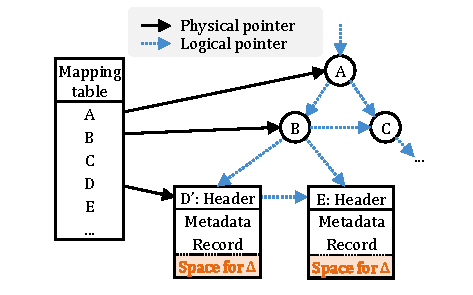
\includegraphics{./figures/Bc-structure.pdf}
    \caption{\Bctree{}の概形}
    \label{fig:bc_tree-structure}
\end{figure}

\subsubsection{データ構造の概観}
\Bptree{}と同様に,\Bctree{}は索引層およびデータ層によって構成される.
索引層のノード(中間ノード)は分割キーと子ノードへのポインタの組を格納し,木の下方への検索を補助する.
構造は\Blinktree{}~\cite{tods1981:Lehman}に則っており,各ノードが同じ階層の右兄弟への参照リンクを持つ.

ノード間の繋がりはマッピングテーブルにより仮想化する.
各ノードは自身の子ノードや兄弟ノードへのポインタを直接持つ代わりにマッピングテーブル上のIDを持つ.
各ノードへの参照はマッピングテーブルを用いた間接参照を採用し,マッピングテーブル内の物理ポインタを差し替えることでそのノードへの参照を一括で変更する.

各ノードの領域は不変領域と可変領域(ノード内バッファ)に分けられる.
不変領域はノードヘッダおよびソート済みのレコードを格納する.
ヘッダは不変領域の情報を管理し,構造変更時のみその値が変更される.
可変領域はステータスワードの格納と差分レコードを挿入するための書き込みバッファの役割を果たす.
ステータスワードは可変領域の情報を管理し,ノードの現在の状態や残容量などを管理する.

\subsubsection{レコード操作の概観}
ステータスワードをCAS命令で更新することによって,ロックフリーな書き込みを実現している.
書き込み操作は差分レコード領域の予約とレコード挿入および可視化の2ステップで行われる.
\Fig{\ref{fig:bc_tree_insertion}}に\Bctree{}における差分レコードの挿入を示す.

ノードフッタには可変領域の状態を表すステータスワードを用意し,この中のレコード数と使用済みブロックサイズを加算することで差分レコード用の領域を予約する.
また,\Bctree{}ではノードの生成時に可変領域をゼロ埋めしている.
\Bctree{}では,メタデータがゼロ埋めされている場合を処理途中として表すため,差分レコード用の領域を予約した時点ではレコードが可視化されていないことを認識できる.
確保した領域へ差分レコードを書き込み,対応するレコードメタデータの値を更新することでレコードを可視化し,挿入処理を完了する.
書き込み同士の競合はステータスワードで解決され,差分レコード用領域の予約,つまり差分レコードの書き込み順はCAS命令の成功順によって順序付けられる.

\begin{figure}[t]
    \centering
    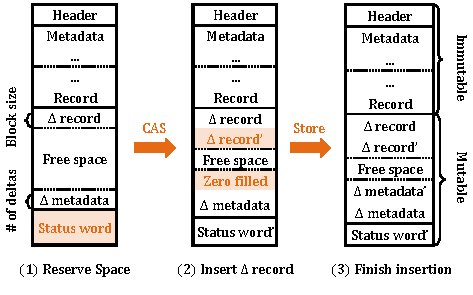
\includegraphics{./figures/Bc-insertion.pdf}
    \caption{\Bctree{}における差分レコードの挿入}
    \label{fig:bc_tree_insertion}
\end{figure}

\subsection{Mass木}
Mass木は\Bptree{}を基本単位とした階層構造やレコードメタデータの削除により,キャッシュ効率を改善した索引構造である.
Mass木の概形を\Fig{\ref{fig:masstree}}に示す.

\begin{figure}[t]
    \centering
    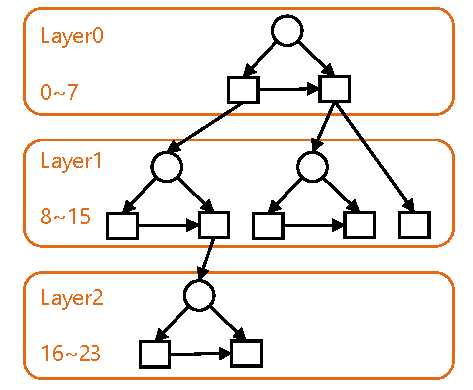
\includegraphics{./figures/masstree.pdf}
    \caption{Mass木の概形}
    \label{fig:masstree}
\end{figure}

Mass木は複数の\Bptree{}とlayer構造から構成される.
Layer~0はキーの先頭0~7~byteで構成される\Bptree{}である.
先頭8~byteで一意性が確保できる場合には,Layer~0で完結する.
先頭8~byteで一意性が確保出来ない場合,Layer~1(キーの8~15~byte目で構成される\Bptree{})を作成し,Layer~0からLayer~1への物理リンクを張る.
同様にして,複数の\Bptree{}やLayerを作成し,トライ木に似た構造を持つのがMass木の特徴である.
Mass木は,整数型や文字列型など先頭からのバイナリ比較で大小判定可能なキーのみを対象とすることで,上記に示す階層化(共通部分の集約)を可能にしている.

また,Mass木は固定長キーおよび固定長ペイロードに特化したノードレイアウトを利用している.
\Bctree{}のような可変長キーおよび可変長ペイロードに対応する索引構造では,各レコードに対応するレコードメタデータを利用することでノード内のレコードの配置等を管理している.
一方,Mass木ではキーを8~byte毎に分割するため各階層の\Bptree{}で管理されるキーが8~byte固定長となる.
ペイロードに関しても,可変長のペイロードなどは動的に確保した領域に保持し索引内にはそのポインタのみを格納することで,索引内では全てのペイロードを同じく8~byte固定長で扱う.
つまりレコードの個数などから一意に参照先を決定でき,レコードメタデータの除外とそれによるCPUキャッシュ効率の改善が実現されている.

\section{\Bcforest{}の構造}
\label{sec:bc_forest_structure}

\Bcforest{}は\Bctree{}をバイナリ比較可能なキーに最適化した索引構造である.
Mass木のように8~byte単位でキーを分割,階層分けし,各階層でのレコード管理にはBc木を利用する.
つまり,各Bc木の中間ノードでは固定長の部分キーおよび子ノードへのポインタのみを管理することとなり,レコードメタデータの除外によるキャッシュ効率の改善が可能となる.
一方で,葉ノードではposting listを用いて共通する部分キーを持つレコードを管理し,少数のレコードのみからなる下層の生成を抑制する.

\subsection{中間ノードにおけるレコードメタデータの除外}
\Bcforest{}ではMass木同様,中間ノードにおいてレコードメタデータを除外できる.
\Fig{\ref{fig:inner}}に,\Bctree{}および\Bcforest{}の中間ノードを示す.
\Bcforest{}ではキーを8~byteで分割しているため、中間ノード中では固定長キーとして扱える.
また,ペイロードは子ノードへのポインタであるため固定長である.
つまり中間ノード内のレコードはメタデータに依らずアクセス可能であり,キャッシュ効率の改善およびそれに伴う索引層の探索性能改善が可能である.

\begin{figure}[t]
    \centering
    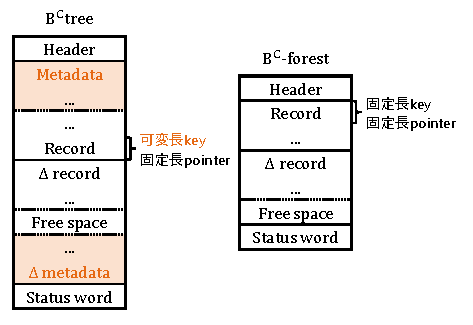
\includegraphics{./figures/inner_node.pdf}
    \caption{\Bcforest{}中間ノードにおけるレコードメタデータの除外}
    \label{fig:inner}
\end{figure}

レコードメタデータの除外に伴い,各レコードの可視および削除済みフラグを子ノードポインタ用の領域で管理する.
メタデータはレコードの配置管理以外に,差分レコードが挿入ないし削除済みであるかどうか判別する役割を担っている.
そのため,メタデータを除外するには各フラグを何らかの方法で管理しなければならない.
そこで,主要OSの仮想メモリの管理において,ユーザ領域の上位bitが未使用であることを利用する~\cite{url:Linux}.
つまり,子ノードへのポインタをレコード中に格納するとき,最上位bitをvisibilityフラグ,2番目のビットをdeletedフラグとして利用する.

\subsection{葉ノードにおけるposting listの導入}
\Bcforest{}では空間利用率の改善として,posting listを導入する.
\Fig{\ref{fig:posting_list}}はposting listを導入した際の索引構造を示したものである.

posting listでは,1~つのキーに対して複数のペイロードを保持できる.
layer~1においてposting list作成することで,layer~2の無駄な階層化と空間利用率の悪化を防ぐ.
なお,posting listは後述する統合時に不変領域に生成され,可変領域には生成しない.

\begin{figure}[t]
    \centering
    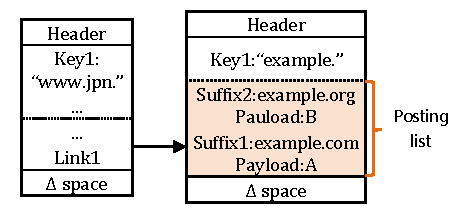
\includegraphics{./figures/posting_list.pdf}
    \caption{posting listの導入}
    \label{fig:posting_list}
\end{figure}

\section{\Bcforest{}のノード操作}
\label{sec:node_operation}
\Bcforest{}は読み取り操作(read,scan)および書き込み操作(upsert,insert,update,delete)をサポートする.
本節では,読み取り操作(read)および書き込み操作(upsert)について説明する.

ノード操作は対象ノードの特定とノード内操作の2段階に分けられる.
対象ノードの特定では,与えられた対象キーをもとに操作対象のノードを特定する.
まず,対象キーの先頭0~7~byteをもとに属するの葉ノードを根ノードから二分探索により特定する(Layer~0).
次に,葉ノード内の不変領域を二分探索し,接頭辞8~byteが共通するキーについて下層へのポインタの有無を確認する.
ポインタが無い場合,本葉ノードを挿入先の葉ノードとして特定する.
ポインタがある場合,下層の根ノードへ移動し,対象キーの8~15~byte目をもとに属する葉ノードを二分探索により特定する(Layer~1).
同様に下層ポインタの有無を確認し,本操作を下層ポインタがなくなるまで繰り返し,葉ノードを特定する.
特定した葉ノード不変領域内に対象キーが一致するレコードがある場合には,その位置を保持し,後述するノード内操作時に利用する.

\subsection{読み取り(read)}
% 読み取り操作の概要と可変領域での読み取り
読み取り(read)は与えられた対象キーのペイロードを返す操作である.
操作対象の葉ノード特定後,葉ノード内の可変領域の線形探索と不変領域の2ステップで読み取り操作を行う.
最新の値は差分レコード領域に書き込まれるため,まず可変領域を線形探索し,一致するキーがあるか確認する.
このとき,差分レコードの数はステータスワードから読み取り,差分レコードが可視化されていなければスキップする.

% 可変領域にレコードがない場合
差分レコード中に対象のレコードが存在しなければ,対象ノードの特定時に保持した位置をもとに,不変領域の読み取りを行う.
接頭辞8~byteが共通するキーについてposting listが存在する場合には,posting list内を線形探索し,接尾辞が一致するキーがあるか確認する.
先頭ノードが構造変更操作の途中である場合には,差分レコードを読み終わった時点で物理ポインタをたどり古いノードへ移動し,同様の2ステップを古いノード上で行う.

% Bc木における読み取り操作の特徴
読み取り処理はwait-freeに動作する.
上述したとおり読み取り命令は一切ノードの状態を変更せず,読み取った状態に応じて適切な手続きを選択する.
そのため,読み取り命令においてリトライなどは発生せず,有限時間内で必ず処理が終了する.

\subsection{書き込み(upsert)}
% 書き込み操作の概要
書き込み(upsert)は与えられた対象キーおよびペイロードを挿入する操作である.
操作対象の葉ノード特定後,posting listチェックとレコード挿入の2ステップで書き込み操作を行う.
\Bcforest{}における書き込み操作では,差分レコードのメタデータにposting listのサイズを持たせる.
これは後述する下層生成操作と書き込み操作の衝突時に,書き込み先ノードを特定するためである.

Posting listチェックでは,キーの一意性を確認する.
読み取り操作と同様に可変領域,不変領域の順に探索し,挿入するレコードを含めたposting listのサイズを計算する.
以上の操作にて,取得したposting listのサイズをメタデータに入れ,\Fig{\ref{fig:bc_tree_insertion}}に示す\Bctree{}と同様の操作で挿入する.

% 書き込みができない場合の対処
以上の書き込み操作によって差分レコードを挿入していくが,挿入後の差分レコードの総数またはノード容量のしきい値を越える場合,構造変更操作が行われる.
しきい値の確認はステータスワードの更新時に行われ,しきい値を越えた場合はレコードの書き込み後にいずれの構造変更操作を行うか判定する.
書き込み処理の大部分はロックフリーに動作するが,後述する構造変更操作の一部手続きとのみロックに基づく制御を利用する.

\section{\Bcforest{}の構造変更操作}
\label{sec:smo}
\Bcforest{}は構造変更操作として差分レコードのノードへの統合(consolidate)とノードの分割(split),併合(merge)および下層生成,下層削除操作を持つ.
本節では統合操作,分割操作および下層生成操作について述べる.

構造変更操作を始める前に,新たなノードをマッピングテーブルに挿入する.
構造変更中に行われる書き込みについては,用意した新たなノード領域に書き込むことで,他のスレッドの待ち時間を削減する.

\subsection{統合}
% 統合操作の概要
統合操作は差分レコードの数またはノードの容量がそれぞれのしきい値を越えた場合,差分レコードと不変レコードをソートして不変領域に反映する操作である.
本操作時に接頭辞8~byteが共通するキーを集約し,不変領域にposting list(3.2節)を作成する.
統合操作を行うことで,可変領域を確保し新たな差分レコードの挿入を受け付ける.

% 統合操作の具体的な手順
\Fig{\ref{fig:bc_tree_consolidastion}}に\Bcforest{}における統合操作を示す.
統合が必要になった場合,新たなノード領域を用意する.
そして,古いノードのステータスワードを更新後,ノードヘッダの情報から統合後に必要な不変領域を計算する.
なお,このステータスワードの更新により古いノードは全体が不変となり,新たな差分レコードは挿入できなくなる.
次に,新たなノードにおいてステータスワードを含むヘッダ情報のみを更新した後,新規ノードとしてマッピングテーブル上の参照を更新する.
その後,古いノード上の差分レコードを不変レコードへ反映させつつ,新たなノードへレコードをコピーする.
最後に,統合後の状態でノードヘッダを更新し,新しいノードにおける不変領域を可視化する.
この際に,後述する分割操作で用いられる分割キーを,統合後のノードの不変領域から計算する.

\begin{figure}[t]
    \centering
    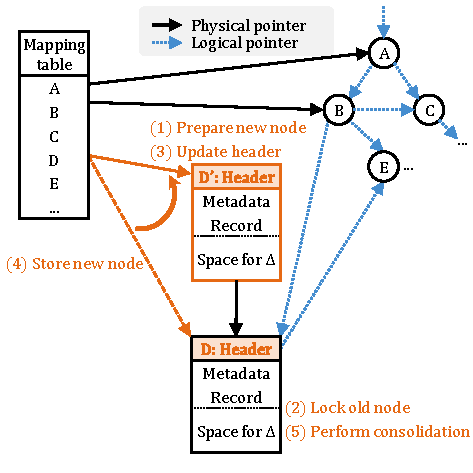
\includegraphics{./figures/Bc-consolidate.pdf}
    \caption{\Bcforest{}における統合操作}
    \label{fig:bc_tree_consolidastion}
\end{figure}

% 統合操作時の書き込みについて
統合操作を行っている際に,発生した書き込み操作は新規ノードの可変領域で受け付ける.
これにより統合操作の間も,読み取り操作は新規レコードの可変領域,統合前のノードの可変領域および不変領域の順でレコードを確認することで読み取り操作を実行できる.

\subsection{分割}
% 分割操作の概要
分割操作はノードの差分レコードの数またはノード容量がそれぞれしきい値を越えており,統合後も十分な可変領域を確保できない場合に,そのノードのレコードを新規の2つのノードに分散させる操作である.
分割操作により,容量が一杯になったノードを2つに分け,新たな差分レコードの挿入を受け付ける.

% 分割操作の具体的な手順
\Fig{\ref{fig:bc_tree_split}}に\Bcforest{}における分割操作を示す.
構造変更操作が必要になった場合,新たなノード領域を2つ用意する.
ステータスワードの更新により対象ノード全体を不変状態にした後,レコードコピーを始める前に用意したノードをマッピングテーブルに挿入する.
これを実現するために,各ノードは自身の分割キーの位置を統合および分割操作のたびに記録する.
分割したノードの挿入後,統合操作と同様の手続きでレコードをコピーする.
分割時には,古いノードの分割キー未満の全てのレコードを左ノードにコピーする.
残りのレコード,すなわち分割キー以上の全てのレコードは右ノードにコピーする.

\begin{figure}[t]
    \centering
    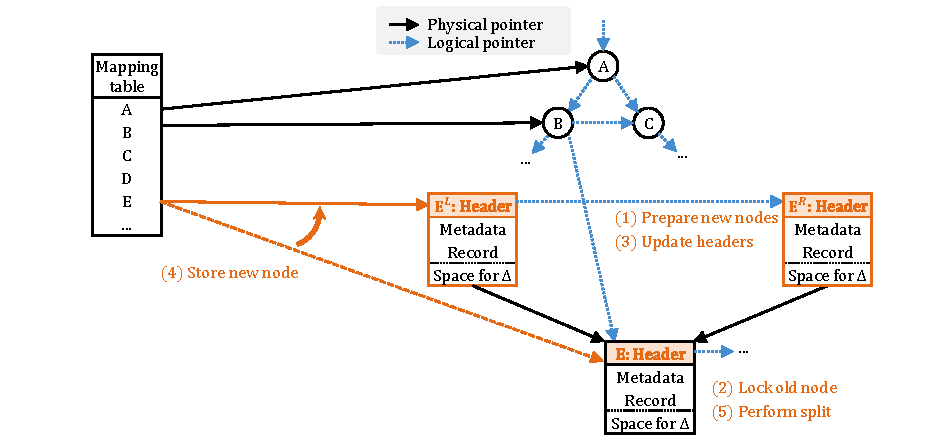
\includegraphics{./figures/Bc-split.pdf}
    \caption{\Bcforest{}における分割操作}
    \label{fig:bc_tree_split}
\end{figure}

% 右子ノードのリンクの反映の遅延
レコードのコピー後は,親ノードに右分割ノードへのリンクを挿入することで分割操作が完了する.
このとき,親ノードへはリンクの情報のみを挿入し,反映は親ノードの統合操作時に行う.
例えば新規ノードEを挿入した際,差分レコード領域に子ノードへのリンク情報のみを追記し統合操作が行われるまでそのリンクの反映を遅延する.
つまり,索引の探索中において中間ノードでは差分レコードを確認せず,不変領域のレコードのみを検索する.

\subsection{下層生成}
% 下層生成操作の概要
下層生成操作はノードの差分レコードの数またはノード容量がそれぞれしきい値を越えており,統合後も十分な可変領域を確保できない場合に,posting list内のレコードを下層に移行する操作である.
下層生成操作により,ノード内のレコードの一部を下層に移行させるとともに,新たな差分レコードの挿入を受け付ける.

\begin{figure}[t]
    \centering
    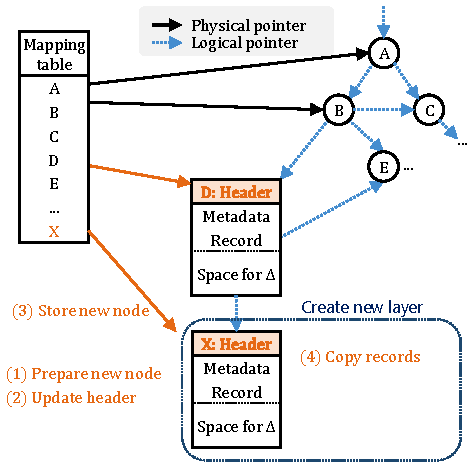
\includegraphics{./figures/layer.pdf}
    \caption{\Bcforest{}における下層生成操作}
    \label{fig:bc_tree_layer}
\end{figure}

% 下層生成操作の具体的な手順
\Fig{\ref{fig:bc_tree_layer}}に\Bcforest{}における下層生成操作を示す.
下層生成操作が必要になった場合,新たなノード領域を用意する.
レコードコピーを始める前に用意したノードをマッピングテーブルに挿入する.
下層生成操作を引き起こすきっかけとなった,posting listのレコードを新たなノードにコピーする.
この時,接尾辞の先頭8~byteをもとに必要であればposting listの作成を行う.
元ノードのposting listがあったペイロード領域に新ノードへのポインタを格納する.

% 下層生成操作時の書き込みについて
下層生成操作を行っている際に書き込み操作が発生した場合,下層生成の有無を確認する.
書き込み操作の一意性チェック時に,posting listのサイズから下層が生成されるか確認する.
生成されない場合は,元ノードに差分レコードを挿入する.
生成される場合は,下層生成操作が終わるまで書き込みはブロックされる.

\section{おわりに}
\label{sec:conclusion}
本稿では\Bctree{}にMass木と同様のトライ木構造を適応させた\Bcforest{}について提案し,その構造および操作を紹介した.
今後は提案した索引構造を実装するとともに,Mass木や近年提案されているBw木やBz木といったロックフリー索引との性能を比較検証する.